%% bare_conf.tex
%% V1.3
%% 2007/01/11
%% by Michael Shell
%% See:
%% http://www.michaelshell.org/
%% for current contact information.
%%
%% This is a skeleton file demonstrating the use of IEEEtran.cls
%% (requires IEEEtran.cls version 1.7 or later) with an IEEE conference paper.
%%
%% Support sites:
%% http://www.michaelshell.org/tex/ieeetran/
%% http://www.ctan.org/tex-archive/macros/latex/contrib/IEEEtran/
%% and
%% http://www.ieee.org/

%%*************************************************************************
%% Legal Notice:
%% This code is offered as-is without any warranty either expressed or
%% implied; without even the implied warranty of MERCHANTABILITY or
%% FITNESS FOR A PARTICULAR PURPOSE! 
%% User assumes all risk.
%% In no event shall IEEE or any contributor to this code be liable for
%% any damages or losses, including, but not limited to, incidental,
%% consequential, or any other damages, resulting from the use or misuse
%% of any information contained here.
%%
%% All comments are the opinions of their respective authors and are not
%% necessarily endorsed by the IEEE.
%%
%% This work is distributed under the LaTeX Project Public License (LPPL)
%% ( http://www.latex-project.org/ ) version 1.3, and may be freely used,
%% distributed and modified. A copy of the LPPL, version 1.3, is included
%% in the base LaTeX documentation of all distributions of LaTeX released
%% 2003/12/01 or later.
%% Retain all contribution notices and credits.
%% ** Modified files should be clearly indicated as such, including  **
%% ** renaming them and changing author support contact information. **
%%
%% File list of work: IEEEtran.cls, IEEEtran_HOWTO.pdf, bare_adv.tex,
%%                    bare_conf.tex, bare_jrnl.tex, bare_jrnl_compsoc.tex
%%*************************************************************************

% *** Authors should verify (and, if needed, correct) their LaTeX system  ***
% *** with the testflow diagnostic prior to trusting their LaTeX platform ***
% *** with production work. IEEE's font choices can trigger bugs that do  ***
% *** not appear when using other class files.                            ***
% The testflow support page is at:
% http://www.michaelshell.org/tex/testflow/



\documentclass[conference]{IEEEtran}
% Add the compsoc option for Computer Society conferences.
%
% If IEEEtran.cls has not been installed into the LaTeX system files,
% manually specify the path to it like:
% \documentclass[conference]{../sty/IEEEtran}


% Some very useful LaTeX packages include:
% (uncomment the ones you want to load)

% *** GRAPHICS RELATED PACKAGES ***
%
\usepackage[pdftex]{graphicx}

% *** MATH PACKAGES ***
%
\usepackage[cmex10]{amsmath}

% *** SUBFIGURE PACKAGES ***
%\usepackage[tight,footnotesize]{subfigure}
% subfigure.sty was written by Steven Douglas Cochran. This package makes it
% easy to put subfigures in your figures. e.g., "Figure 1a and 1b". For IEEE
% work, it is a good idea to load it with the tight package option to reduce
% the amount of white space around the subfigures. subfigure.sty is already
% installed on most LaTeX systems. The latest version and documentation can
% be obtained at:
% http://www.ctan.org/tex-archive/obsolete/macros/latex/contrib/subfigure/
% subfigure.sty has been superceeded by subfig.sty.



%\usepackage[caption=false]{caption}
\usepackage[font=footnotesize,caption=false]{subfig}
% subfig.sty, also written by Steven Douglas Cochran, is the modern
% replacement for subfigure.sty. However, subfig.sty requires and
% automatically loads Axel Sommerfeldt's caption.sty which will override
% IEEEtran.cls handling of captions and this will result in nonIEEE style
% figure/table captions. To prevent this problem, be sure and preload
% caption.sty with its "caption=false" package option. This is will preserve
% IEEEtran.cls handing of captions. Version 1.3 (2005/06/28) and later 
% (recommended due to many improvements over 1.2) of subfig.sty supports
% the caption=false option directly:
%\usepackage[caption=false,font=footnotesize]{subfig}
%
% The latest version and documentation can be obtained at:
% http://www.ctan.org/tex-archive/macros/latex/contrib/subfig/
% The latest version and documentation of caption.sty can be obtained at:
% http://www.ctan.org/tex-archive/macros/latex/contrib/caption/


% --------------- USEPACKAGE agregados por guanucoluis ----------------

\usepackage[utf8]{inputenc}
\usepackage{multirow}
%\usepackage[english]{babel}
\usepackage{amssymb}
%\usepackage[pdftex]{graphicx}
\usepackage[hyphenbreaks]{breakurl}
\usepackage[hyphens]{url}
\usepackage{lipsum}

% ------------------------- Agregados por maxi ------------------------

\renewcommand{\abstractname}{Resumen}
\renewcommand{\IEEEkeywordsname}{Palabras claves}
\renewcommand{\figurename}{Fig.}
\renewcommand{\tablename}{Tabla}
\renewcommand{\refname}{Referencias}
\hyphenation{de-sa-rro-llar de-sa-rro-llos}

%lista de posibles "Fixed names"  de latex que pueden hacer falta
%\abstractname	 Abstract
%\alsoname	 see also (makeidx package)
%\appendixname	 Appendix
%\bibname	 Bibliography (report,book)
%\ccname	 cc (letter)
%\chaptername	 Chapter (report,book)
%\contentsname	 Contents
%\enclname	 encl (letter)
%\figurename	 Figure (for captions)
%\headtoname	 To (letter)
%\indexname	 Index
%\listfigurename	 List of Figures
%\listtablename	 List of Tables
%\pagename	 Page (letter)
%\partname	 Partnnn
%\refname	 References (article)
%\seename	 see (makeidx package)
%\tablename	 Table (for caption)



% correct bad hyphenation here
\hyphenation{op-tical net-works semi-conduc-tor}


\begin{document}
%
% paper title
% can use linebreaks \\ within to get better formatting as desired
\title{Servicios REST}


% author names and affiliations
% use a multiple column layout for up to three different
% affiliations
\author{\IEEEauthorblockN{Franco Bocalon, Luis Guanuco, Santiago
    Nolasco}
  \IEEEauthorblockA{Sistemas Distribuidos\\
    Especialidad en Sistemas Embebidos\\
    Instituto Universitario Aeronáutico}
}

% use for special paper notices
%\IEEEspecialpapernotice{(Invited Paper)}


% make the title area
\maketitle


\begin{abstract}
  \lipsum[1]
\end{abstract}

% Note that keywords are not normally used for peerreview papers.
\begin{IEEEkeywords}
IEEE, IEEEtran, journal, \LaTeX, paper, template.
\end{IEEEkeywords}

% IEEEtran.cls defaults to using nonbold math in the Abstract.
% This preserves the distinction between vectors and scalars. However,
% if the conference you are submitting to favors bold math in the abstract,
% then you can use LaTeX's standard command \boldmath at the very start
% of the abstract to achieve this. Many IEEE journals/conferences frown on
% math in the abstract anyway.

% no keywords

% For peer review papers, you can put extra information on the cover
% page as needed:
% \ifCLASSOPTIONpeerreview
% \begin{center} \bfseries EDICS Category: 3-BBND \end{center}
% \fi
%
% For peerreview papers, this IEEEtran command inserts a page break and
% creates the second title. It will be ignored for other modes.
\IEEEpeerreviewmaketitle

\section{Introducción}

\lipsum[2-3]

\begin{table}[!t]
\renewcommand{\arraystretch}{1.3}
\caption{Recursos de hardware en función de los niveles de aprendizaje}
\label{tab:rec-plataforma}
\centering
\begin{tabular}{|l|c|c|c|}
\hline
\multirow{2}{*}{Nivel} & Llaves/pulsadores & ADC\&DAC/SPI & USB/ETH \\
                       & Diodos LED & Display LCD/VGA & HDMI \\
\hline
Inicial & $\checkmark$ & & \\
\hline
Medio & $\checkmark$ & $\checkmark$ & \\
\hline
Avanzado & $\checkmark$ & $\checkmark$ & $\checkmark$ \\
\hline
\end{tabular}
\end{table}

\lipsum[3-4]

\begin{figure}[!t]
  \centering
  \subfloat[BASYS2 (Digilent)]{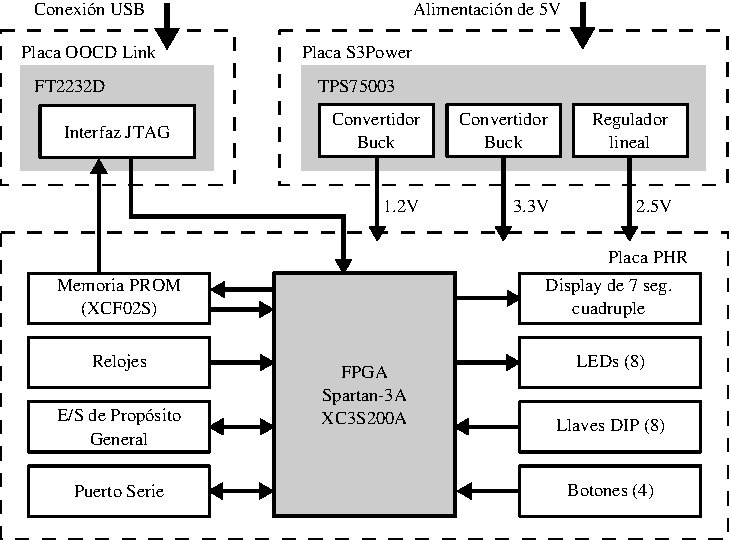
\includegraphics[width=0.2\textwidth]{img/block}%  
    \label{fig:digilent-board}}
  \hfil
  \subfloat[DE0-Nano (Altera)]{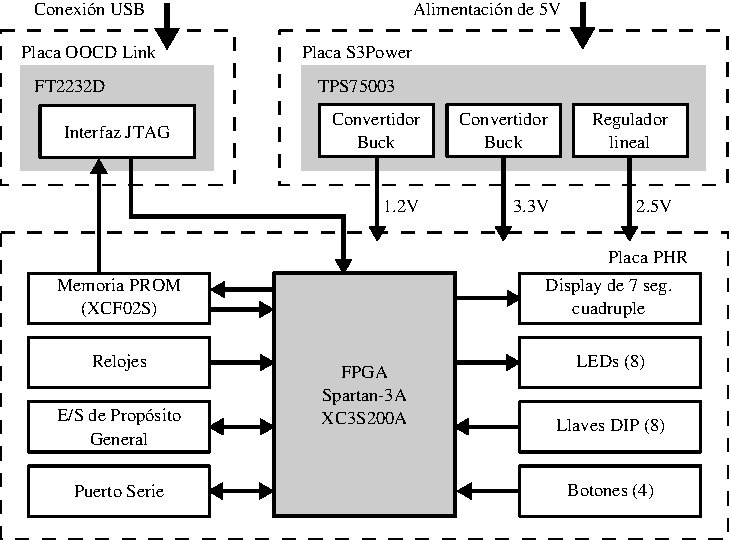
\includegraphics[width=0.2\textwidth]{img/block}%
    \label{fig:altera-board}}
  \hfil
  \subfloat[Avnet Spartan-6 LX150T (Xilinx/Avnet)]{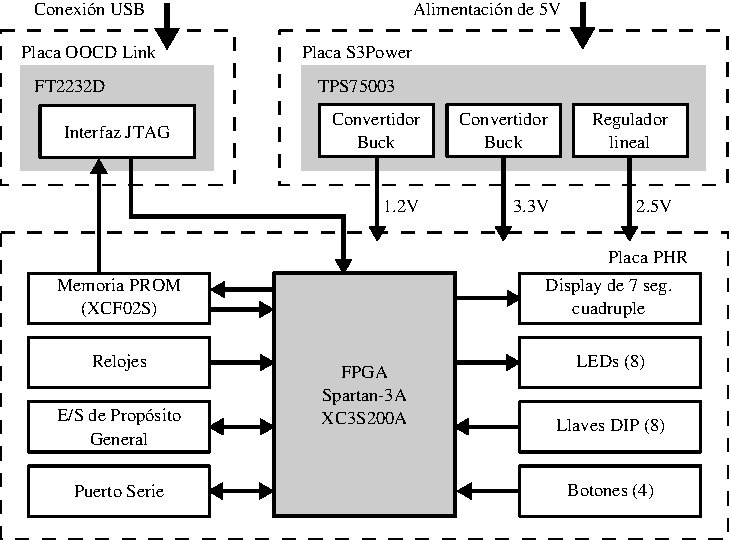
\includegraphics[width=0.2\textwidth]{img/block}%
    \label{fig:xilinx-board}}
  \caption{Plataformas comerciales de desarrollo educativas basadas en FPGAs.}
  \label{fig:board-fpga}
\end{figure}

\lipsum[6]

\section{Dispositivos principales}

\lipsum[7-9]
\subsection{FPGA}
\label{sec:fpga}
La FPGA que se utiliza pertenece a la familia Spartan-3 de Xilinx Inc. Esta familia a la vez se clasifican en

\begin{itemize}
\item Familia Spartan-3A extendida (bajo costo):
  \begin{itemize}
  \item Spartan-3A
    \begin{itemize}
    \item Ideal para uso de interfaz entre dispositivos.
    \end{itemize}
  \item Spartan-3A DSP
    \begin{itemize}
    \item Mayor densidad de recursos en comparación que la familia Spartan-3A
    \item Dispone de un dispositivo DSP (DSP48A)
    \end{itemize}
  \item Spartan-3AN
    \begin{itemize}
    \item Dispositivos no volátiles
    \item Ideal para aplicaciones con restricciones de espacio
    \end{itemize}
  \end{itemize}
\item Familia Spartan-3E
\item Familia Spartan-3
\end{itemize}

\lipsum[10-13]

\begin{table}[!t]
%increase table row spacing, adjust to taste
\renewcommand{\arraystretch}{1.3}
% if using array.sty, it might be a good idea to tweak the value of
% \extrarowheight as needed to properly center the text within the cells
\caption{Característica de la familia Spartan-3A}
\label{tab:char-fpga}
\centering
% Some packages, such as MDW tools, offer better commands for making tables
% than the plain LaTeX2e tabular which is used here.
\begin{tabular}{|l|c|c|c|c|}
\hline
\multirow{2}{*}{\textbf{Devices}} & \textbf{System} & \textbf{Block RAM} & \textbf{Dedicated} &  \textbf{Maximum} \\
 & \textbf{Gates} & \textbf{bits} & \textbf{Multipliers} & \textbf{User I/O} \\
\hline
XC3S50A & 50K & 54K & 3 & 144 \\
\hline
\textbf{XC3S200A} & \textbf{200K} & \textbf{288K} & \textbf{16} & \textbf{248} \\
\hline
XC3S400A & 400K & 360K & 20 & 311 \\
\hline
XC3S700A & 700K & 360K & 20 & 372 \\
\hline
XC3S1400A & 1400K & 576K & 32 & 502 \\
\hline
\end{tabular}
\end{table}

\subsection{Memoria de configuración}
\label{sec:mem-prog}

\lipsum[14-16]

\begin{table}[!t]
\renewcommand{\arraystretch}{1.3}
\caption{Tipo de memoria para la familia Spartan-3A}
\label{tab:mem-fpga}
\centering
\begin{tabular}{|l|c|c|}
\hline
\multirow{2}{*}{\textbf{Devices}} & \textbf{Configuration} & \textbf{ISP PROM} \\
 & \textbf{Bits} & \textbf{Solution} \\
\hline
XC3S50A   & 437,312   & XCF01S \\
\hline                        
\textbf{XC3S200A}  & \textbf{1,196,128} & \textbf{XCF02S} \\
\hline                        
XC3S400A  & 1,886,560 & XCF02S \\
\hline                        
XC3S700A  & 2,732,640 & XCF04S \\
\hline
XC3S1400A & 4,755,296 & XCF08P     \\
\hline
\end{tabular}
\end{table}

\lipsum[20-22]

\section{Sistema de alimentación}
\label{sec:sist-power}

\lipsum[25-27]

\section{Placa PHR}
\label{sec:placa-phr}

\lipsum[30-33]

\begin{figure}[!t]
\centering
  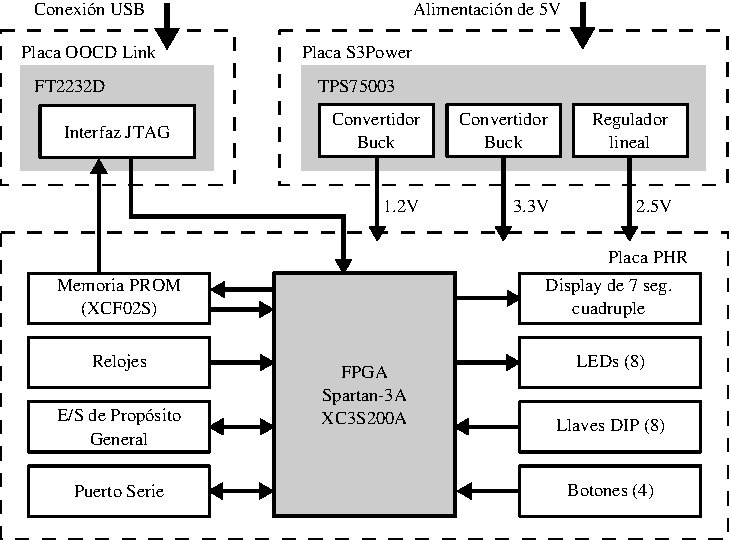
\includegraphics[width=0.45\textwidth]{img/block}
  \caption{Diagrama en bloque de la PHR.}
  \label{fig:phr-bloque}
\end{figure}

\lipsum[35-37]

\begin{figure}[!t]
  \centering
  \subfloat[Placa PHR (base)]{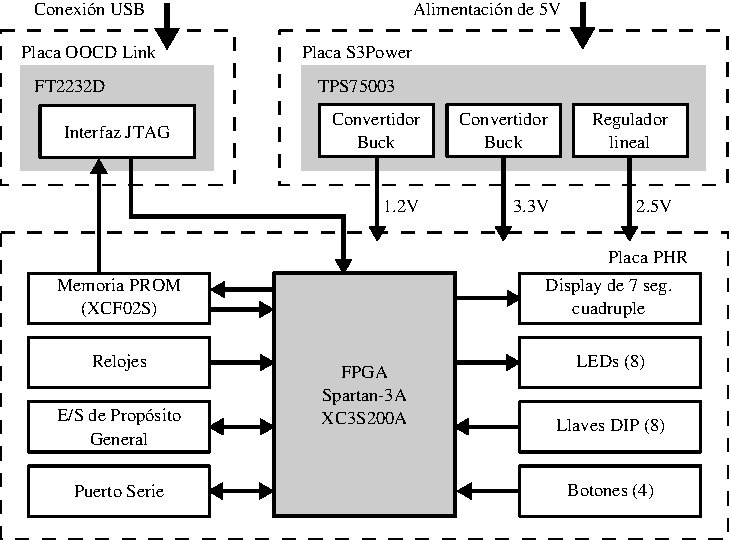
\includegraphics[width=0.4\textwidth]{img/block}%  
    \label{fig:foto-phr}}
  \hfil
  \subfloat[Placa S3Power]{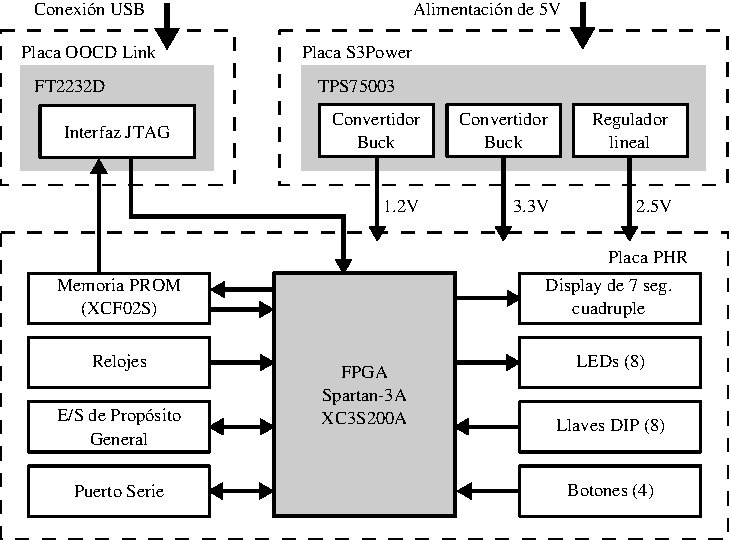
\includegraphics[width=0.2\textwidth]{img/block}%
    \label{fig:foto-s3power}}
  \hfil
  \subfloat[Conexión PHR-S3Power]{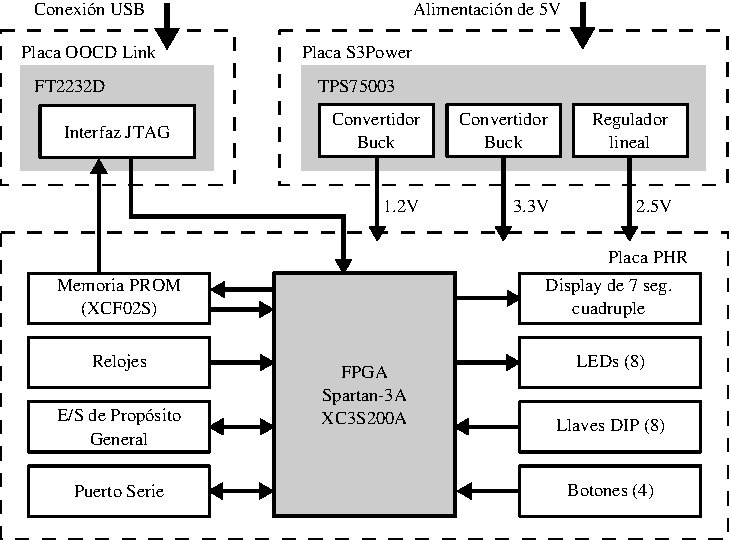
\includegraphics[width=0.25\textwidth]{img/block}%
    \label{fig:foto-phr-s3power}}
  \caption{Placas PHR y S3Power.}
  \label{fig:placas-phr-s3power-con}
\end{figure}

\subsection{Periféricos}
\label{sec:perifericos}

\lipsum[40-43]

\section{Interfaz JTAG}
\label{sec:jtag}

\lipsum[45-48]

\begin{figure*}[!t]
  \centerline{\subfloat[Esquema de la  FT2232D]{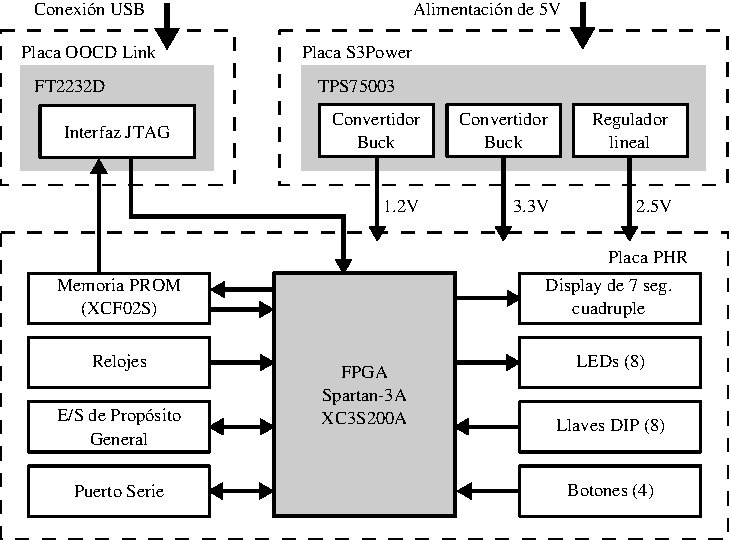
\includegraphics[width=0.35\textwidth]{img/block}%  
    \label{fig:oocdlink-bloque}}
  \hfil
  \subfloat[Placa OOCDLink]{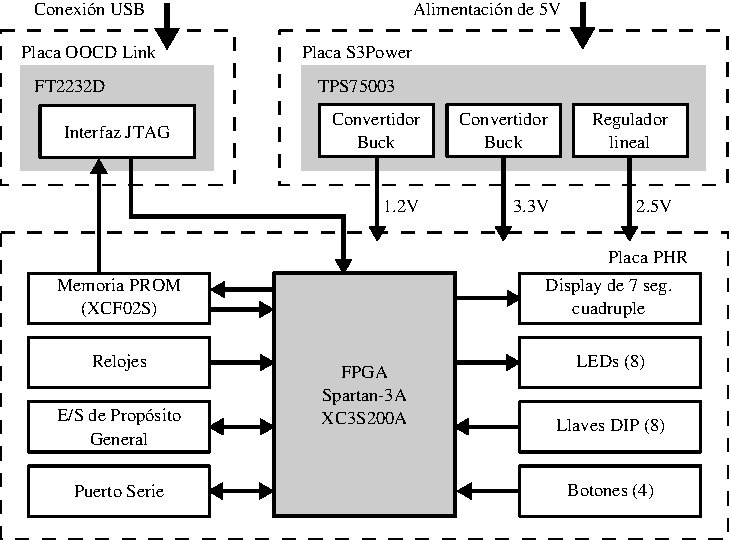
\includegraphics[width=0.2\textwidth]{img/block}%
    \label{fig:oocdlink-foto}}
  \hfil
  \subfloat[Conexión entre la placa PHR y OOCDLink]{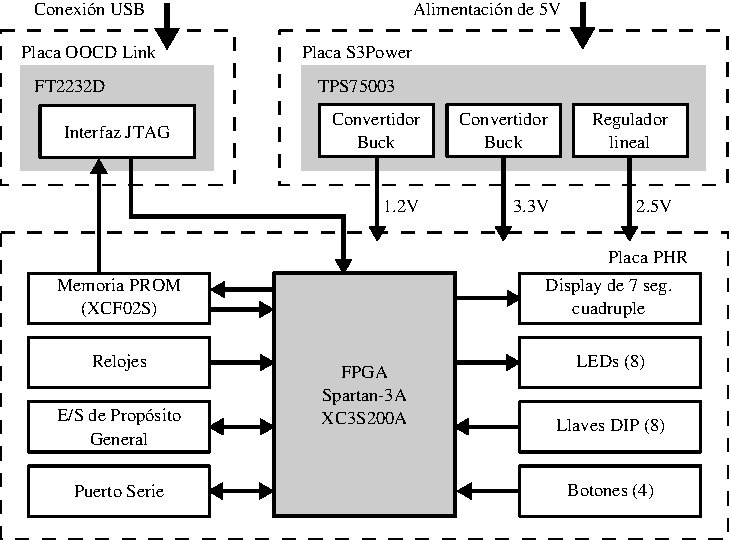
\includegraphics[width=0.4\textwidth]{img/block}%
    \label{fig:oocdlink-phr}}}
  \caption{Interfaz JTAG (implementación FT2232D).}
  \label{fig:oocdlink}
\end{figure*}

\section{Proceso de configuración y programación}

\lipsum[50-53]

\subsection{PHR GUI}

\lipsum[55-58]

\begin{figure}[!t]
\centering
  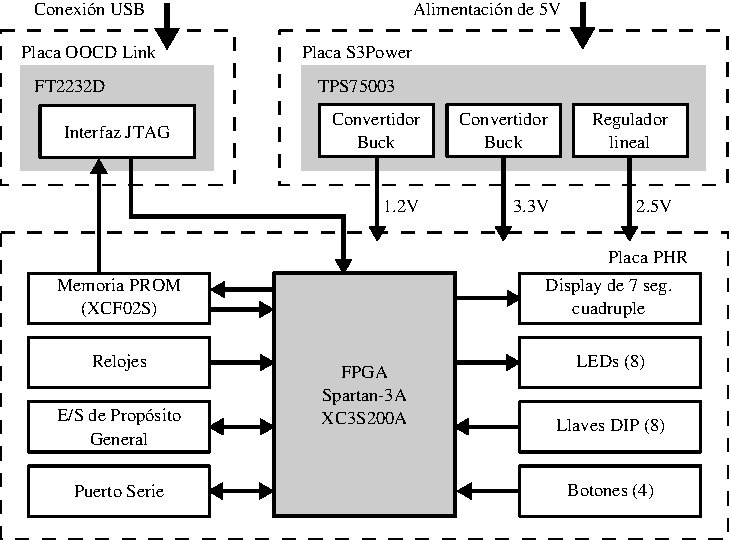
\includegraphics[width=0.4\textwidth]{img/block}
  \caption{Captura de pantalla del software PHR GUI.}
  \label{fig:flujo-hdl}
\end{figure}


\section{Discusión}

\subsection{Costos}
\label{sec:costos}

\lipsum[60-64]

\subsection{Disposiciones del sistema de alimentación}
\label{sec:disp-sistem-alim}

\lipsum[66-69]

\section{Conclusiones}

\lipsum[70-73]

\section*{Agradecimientos}

\lipsum[75-80]

\begin{thebibliography}{1}

% \bibitem{IEEEhowto:kopka}
% H.~Kopka and P.~W. Daly, \emph{A Guide to \LaTeX}, 3rd~ed.\hskip 1em plus
%   0.5em minus 0.4em\relax Harlow, England: Addison-Wesley, 1999.

\bibitem{ASArev.1}
Hiroyuki~Ochi, \emph{ASAver.1: An FPGA-Based Education Board for
  Computer Architecture/system Design}, Design Automation Conference
1997. Proceedings of the ASP-DAC'97. Asia and South Pacific. January
1997.

\bibitem{FPGA-platform-CPU-design}
C.~Chang, C.~Huang, Y.~Lin, Z.~Huang and T.~Hu, \emph{FPGA Platform
  for CPU Design and Applications},  5th. IEEE Conference on
Nanotechnology. Nagoya, Japan. July 2005.

\bibitem{Low-Cost-Interactive-Rapid-Prototyping}
D.~Kang, S.~Hwang, K.~Jhang, K.~Yi, \emph{A Low Cost and Interactive
  Rapid Prototyping Platform For Digital System Design Education},
IEEE International Conference on Microelectronic Systems Education,
MSE'07. 2007. 

\bibitem{FPGA-Based-Experiment-Platform-for-Multi-Core-System}
J.~Xing, W.~Zhao and H.~Hu, \emph{An FPGA-Based Experiment Platform
  for Multi-Cores System}, 9th. International Conference for Young
Computer Scientistis, ICYCS'08. 2008. 

\bibitem{fpgalibre-paper}
S.~Tropea, D.~Brengi, and J.~Borgna, \emph{FPGAlibre: Herramientas de
  software libre para diseño con FPGAs}, FPGA Based Systems. Mar del
Plata: Surlabs Project, 2nd. Southern Conference on Programmable
Logic, 2006.

\end{thebibliography}

% that's all folks
\end{document}


